\documentclass[12pt,a4paper]{article}
\usepackage[width=.75\textwidth]{caption}
\usepackage{graphicx}
\usepackage{authblk}
\usepackage{amsmath}
\usepackage{amsfonts}
\usepackage{braket}
\usepackage{siunitx}
\usepackage{epigraph}
\usepackage{float}
%\usepackage{mathrsfs}
\usepackage[mathscr]{euscript}
\usepackage[top=2cm, bottom=2cm, left=2cm, right=2cm]{geometry}
\usepackage{fancyhdr}

\setlength{\epigraphwidth}{0.8\textwidth}

\pagestyle{fancy}
\begin{document}

%title and author details
\title{Information Theory and Physics of ``Matter Channels''}
\author[1]{Kevin Player\footnote{kjplaye@gmail.com}}

\maketitle

\epigraph{After long reflection in solitude and meditation, I suddenly had the idea, during the year 1923, that the discovery made by Einstein in 1905 should be generalised by extending it to all material particles and notably to electrons.}{Louis de Broglie}

\abstract{We explore information theoretic aspects of matter.  Matter is considered to have a distinct sampling rate and channel capacity, akin to a signal.  We refer to this signal as a ``matter channel''.  We demonstrate how matter channels can be modeled by Dirac spinors.  Finally, we show how to think of proper time as an emergent property of matter.}

\section{The Sampling Rate of Matter}
\label{rate}
We review several results which all point to a ``sampling rate'' of matter.
\subsection{De Broglie Matter Waves}
Almost exactly 100 years ago, De Broglie famously conjectured that matter should have the same kind of wave-like properties that light has.  This was verified using electrons, and then other particles.  The resulting matter waves have a (De Broglie) frequency
\[
  f_{DB} = \frac{E}{h}
\]

\subsection{Bremermann Computational Limit}
While thinking about Heisenberg's uncertainly principle for computation, Bremermann theorized a maximum ``clock-rate'' for a computer.  The argument was to find a minimally physically relevant time resolution for a given mass/energy.  This yielded a universal constant
\[
  C_{Br} = \frac{c^2}{h} \hspace{0.5 in} (\si[per-mode=symbol]{samples\per\kilogram.\sec})
\]
in samples per kilogram per second.  If you multiply this constant by a given mass, we find
\[
 f_{Br} = m C_{Br} = \frac{mc^2}{h} = f_{DB}
\]

\subsection{Zitterbewegung}
Gregory Breit and Erwin Schrödinger studied theoretical oscillations of the electron as it appears in fermionic field theory.  These oscillations were named Zitterbewegung or ``jittery motion'' in German.  The frequency 
\[
 f_{Zitter} = \frac{4 \pi mc^2}{h}
 \]
is off by a factor of $4 \pi$ from $f_{DB}$ and $f_{Br}$ but is otherwise in agreement.  We will come back to this in more detail in Section \ref{ticktock} where the Zitterbewegung frequency matches $f_{DB}$.

\subsection{Samples per Second}
We consider these frequencies to be in
\begin{itemize}
 \item cycles per second ($f_{DB}$),
 \item clocks per seconds ($f_{Br}$),
 \item or field theoretic interactions per second ($f_{Zitter}$)
\end{itemize}
respectively.  But more generically we will just say samples per second. 

\section{Channel Capacity}
\subsection{Bekenstein and Dynamic Range}
Bekenstein found a limiting total amount of information within a given surface area.  Given a sphere radius $R$,  mass $M$, and an entropy $H$ we have
\begin{equation}
\label{bek}
  H \le \frac{2 \pi c R M}{\hbar \ln(2)} \hspace{0.5 in} (\si[per-mode=symbol]{bits})
\end{equation}
The inequality is equality for a black hole where we say that the information is saturated.  When $H$ is less than the right hand side, we still have a channel with entropy given by the right hand side.  It is just only fully ``used'' when $M$ is a black hole.

Let $f$ be the sampling rate of our mass $M$.  Consider a sphere whose radius, $R$, is given by the  the resolution of the mass, the Compton wavelength\footnote{We will see in section \ref{ticktock} how massive particles have instantaneous velocity equal to $c$, so using Compton wavelength is appropriate.}
\[
  R=c/f  
\]
Then the saturated version of (\ref{bek}) yields
\[
 \frac{fH}{M} = \frac{4 \pi^2 c^2}{h \ln(2)} = C_{Bek} \hspace{0.5 in} (\si[per-mode=symbol]{bits\per\kilogram.\sec})
\]
in bits per kilogram per second.

A channel capacity is made up of two things, the number of samples per second and the effective number of bits per sample, the dynamic range.  Section \ref{rate} covered the first part and now we cover the second
\begin{equation}
\label{cap}
   C_{Bek} / C_{Br} = \frac{4 \pi^2}{\ln(2)} \approx 56.96 \hspace{0.5 in} (\si[per-mode=symbol]{bits\per sample})
\end{equation}
which is approximately 7 bytes per sample. 

So the channel capacity is approximately
\[
\text{(7 bytes per sample)} \cdot f_{DB}.
\]

\subsection{Ensembles}
Consider a system with two masses, $m_1$ and $m_2$.  The ensemble system has a mass $m_{12}$ which is the sum of masses
\[
m_{12} = m_1 + m_2.
\]
The samples of the ensemble are just the disjoint union of the samples of $m_1$ and $m_2$.   This is to say that the samples of an ensemble are made up of the samples of all of the components.  In this way, the frequencies add, and we make sense of the linear relationship between mass and frequency.  In a similar way, the channel capacity of the ensemble is the sum of channel capacities of the components, which is to be expected for independent channels.

\section{Proper Time Stream}
An alternative to using (\ref{bek}) can be found by working in the mass's frame of reference. In this frame, the only dimension is time, which we call proper time from general relativity.  We imagine samples as events along the proper time line, see Figure \ref{timeline}.  These zero dimensional samples separate the one dimensional past and future and can be though of as analogs of holographic screens.  

In \cite{thrust}, \cite{entropic}, and \cite{bekenstein}, a particle one wavelength away from a holographic screen was studied.  We are in a reduced dimensional version of that case.  Here we have ``screens'' at each sample on the time line.  The amount of information associated with a particle, one wavelength away, entering a holographic screen was found in \cite{thrust}.  It was $\Delta S = 4\pi^2$, which when compared to a bit, $k \ln(2)$, matches (\ref{cap}).  So we find the same value for the dynamic range of the channel.

%\[
%\begin{array}{c}
%  \Delta S = \frac{4\pi^2}{ln(2)} \\ \approx 56.96 (\si[per-mode=symbol]{bits\per sample})
%\end{array}
%\]

\begin{figure}[H]
\centering
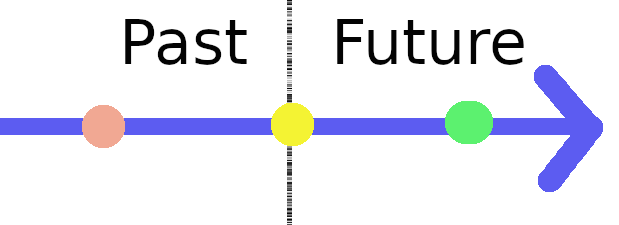
\includegraphics[scale=0.23]{time_line.png}
\caption{A 1-dimensional (proper) time line.  The red, yellow, and green dots are 0-dimensional events, in the past, present and future respectively.  A screen is pictured at the present.}
\label{timeline}
\end{figure}

\section{Zig Zag Particles}
\label{ticktock}
We outline a matter channel picture for an electron in the Dirac field.  There we consider the Dirac equation which involves 4 by 4 matrices and a 4-spinor.  Ryder \cite{ryder} presents the construction of the spinors by considering the Lie algebra of the Lorentz group of symmetries of Minkowski space.  It decomposes into two components for the 2 helicities, counter-clockwise and clockwise.
\[
\mathfrak{so(3,1)} = \mathfrak{su(2)} \times \mathfrak{su(2)}
\]
More specifically, the first $\mathfrak{su(2)}$ is generated by the three coordinate boosts each along with a counter-clockwise twist, whereas the second $\mathfrak{su(2)}$ is generated by the three coordinate boosts each along with a clockwise twist.  These amount to an alternative six generators than the usual three Euclidean rotations and three boosts independently.

Using the Lie algebra decomposition, the Dirac 4-spinor can then be thought of as a system of two 2-spinors with opposite and equal momenta and opposite helicity.  In \cite{penrose}, Penrose carries this farther by suggesting that there could be a physical reality behind this construction.  He proposes that the 2-spinors are moving instantaneously at the speed of light and interact regularly at the De Broglie frequency.  He named these spinors zig-zag particles, and even suggested that the 4-spinor is given mass from the two 2-spinors regularly interacting with the Higgs field and each other.

\begin{figure}[h]
\centering
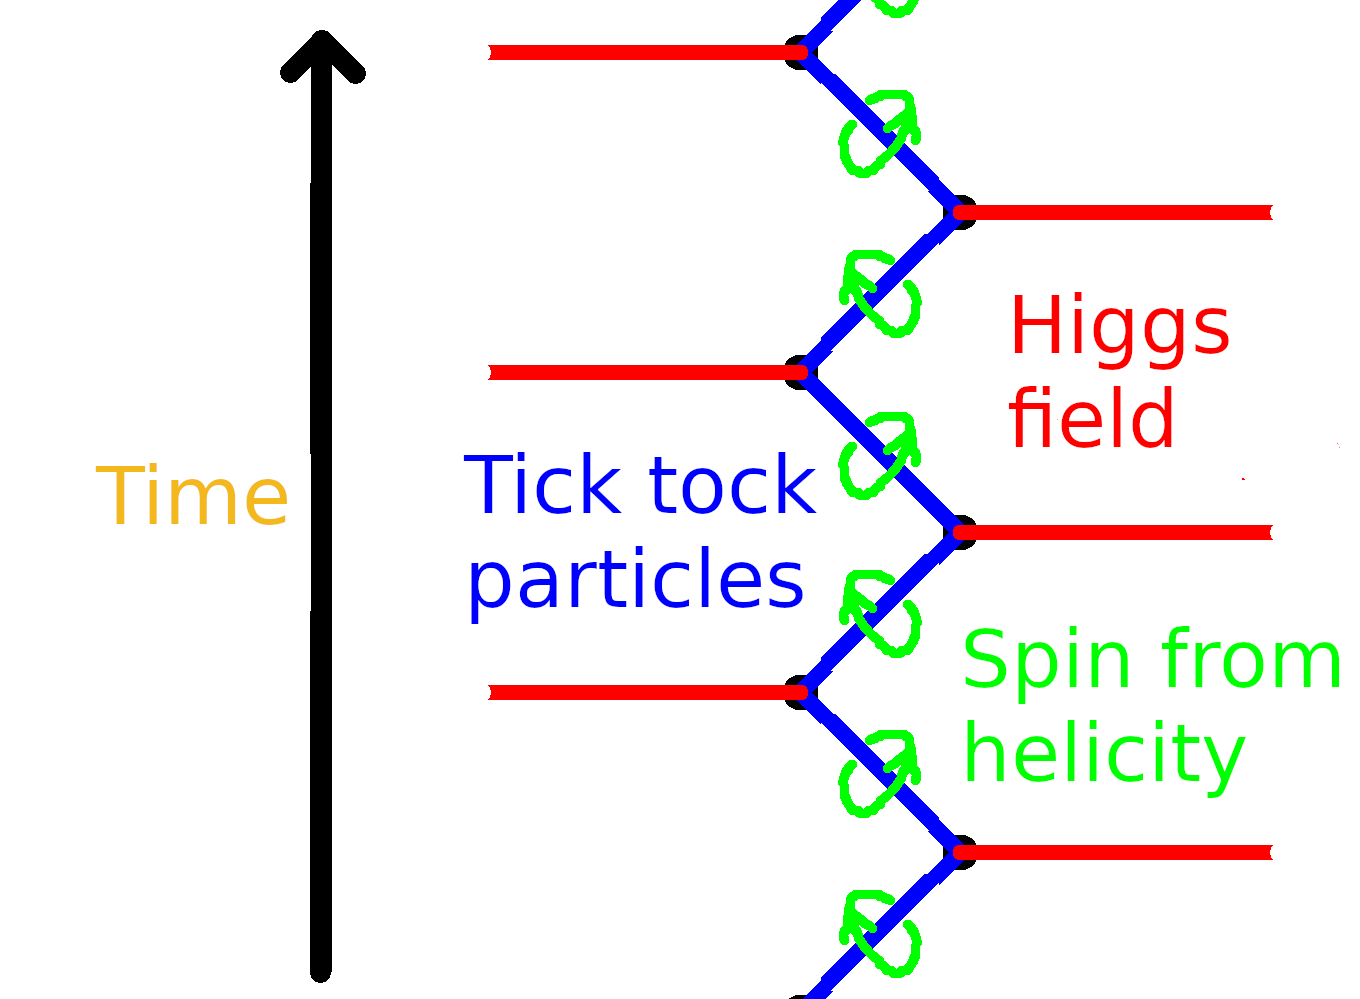
\includegraphics[scale=1.0]{zig_zag_color.png}
\caption{These figures were adapted from \cite{penrose}.  They show his interpretation of the Dirac equation and the Higgs mechanism for an electron.}
\label{zigzag}
\end{figure}

\section{Emergent Proper Time - Tick Tock Particles}
If this mechanism is the origin of mass, we motivate an origin of time as well.  The argument is that time is fundamentally made up of a series of events. The series of events is a series of samples, and is a 1-dimensional ``foliation'', as in \cite{entropic}, of holographic screens. 

The 2-spinors are moving at the speed of light, so they don't interact except at the regular intervals. The only capacity for interaction occurs at these samples and at a fixed rate and dynamic range.  We suggest that the zig-zag particles could have a more suggestive name, as ``tick-tock'' particles, since time as a series of events emerges from this picture.

\section{Prediction}
We predict that a massive particle should be limited by its channel capacity.  It should not be able to receive, store, or transmit information beyond this limitation.

\bibliographystyle{ieeetr}
\bibliography{bibliography}

\end{document}
